
\chapter{Plugin}
\label{chap:results}


\section{How to write a plugin}


The first thing that I looked for in the \umld documentation was how add something in the software. It is a real challenge in software development. Fortunately, I quickly found on the \umld developer Guide, that there is a the developer environment to do that. This environment was an Eclipse environment, which is looking as the figure \ref{fig:eclipse}.

\begin{figure}[h]
  \centering
  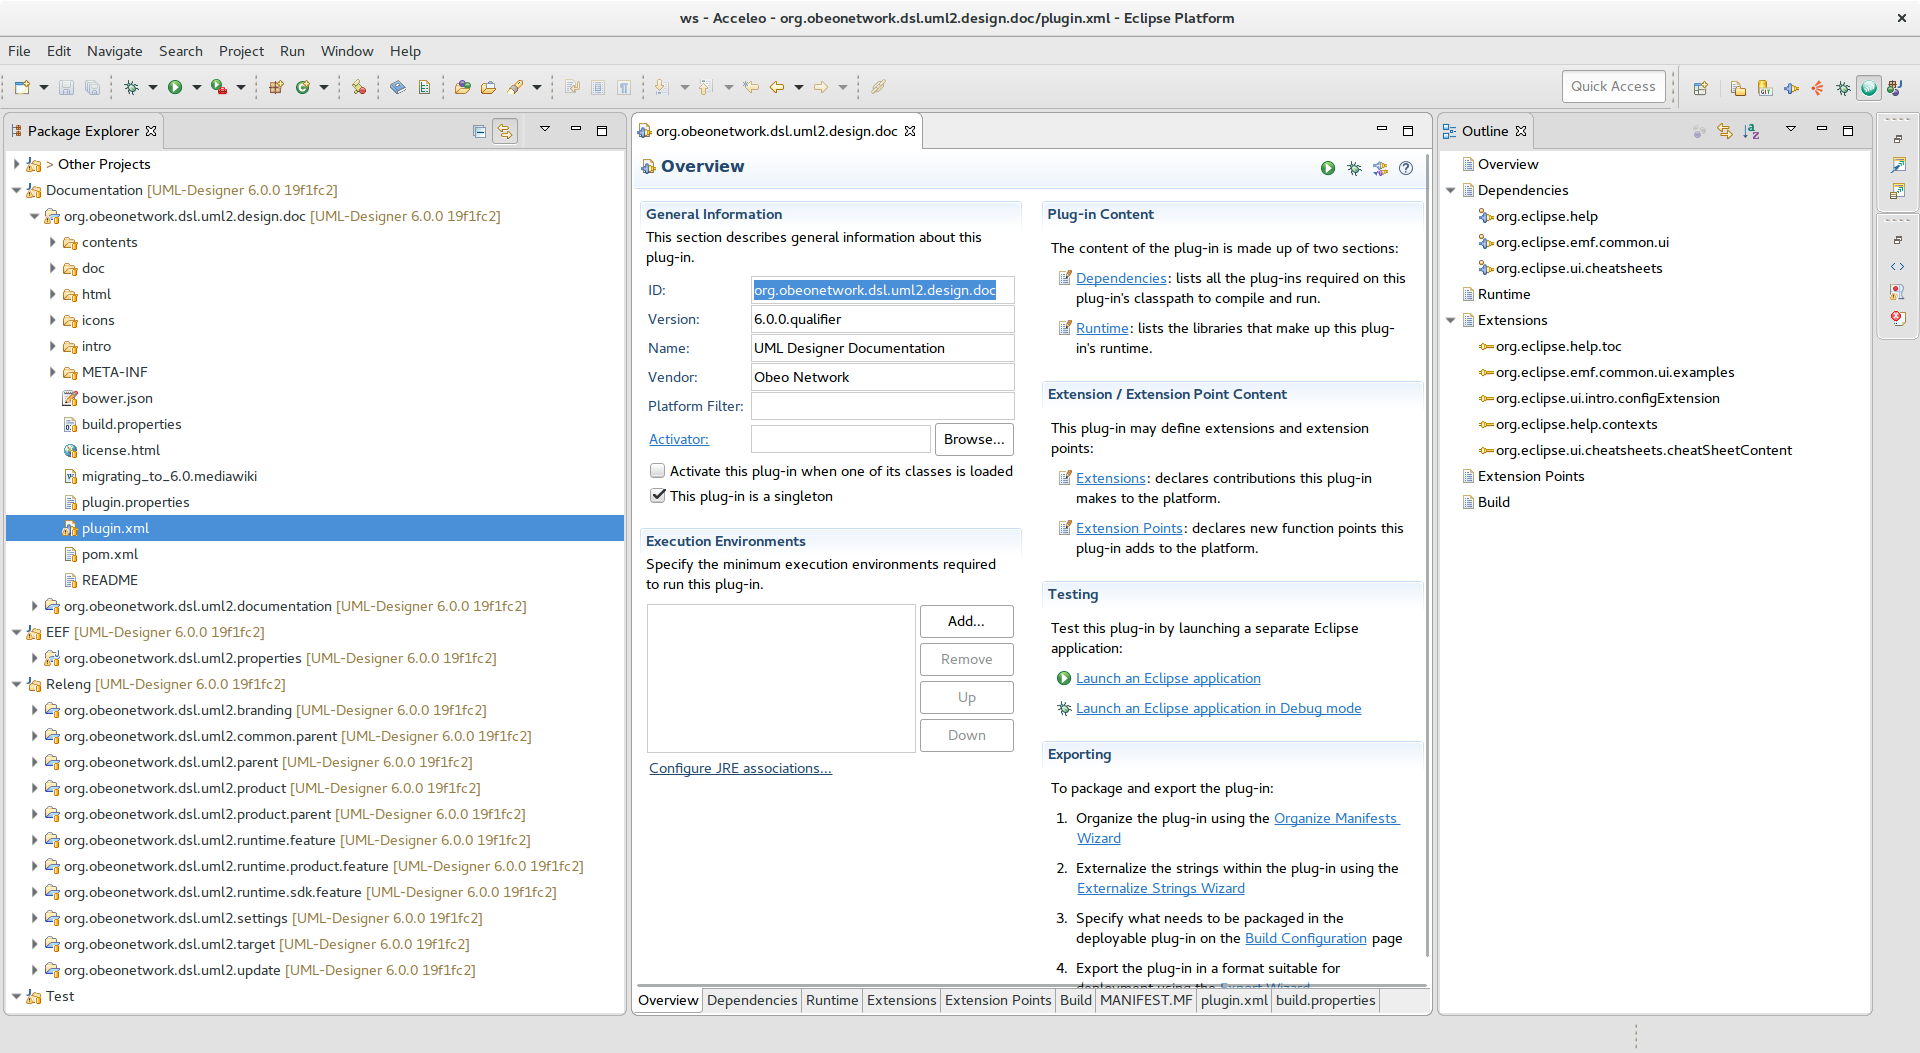
\includegraphics[width=0.8\linewidth]{eclipse}
  \caption{Eclipse environment}
  \label{fig:eclipse}
\end{figure}

Then, I use the fact that \umld is based on Eclipse to create the plugin. The creation of a plugin is the same as an Eclipse plugin. So I made some research on how write an Eclipse plugin. I learn that there is a special structure. This structure permit to keep the modularity and the possibility to install the plugin in all platform. The structure of an eclipse plugin follow the structure show on the figure \ref{fig:plugin}.

\begin{figure}[h]
  \centering
  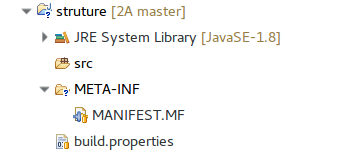
\includegraphics[width=0.5\linewidth]{structure_plugin}
  \caption{Structure of an eclipse plugin}
  \label{fig:plugin}
\end{figure}

\noitemsep
\begin{itemize}
\item The directory \textit{JRE System Library} contains all libraries used to run the plugin
\item The directory \textit{src} contains sources of the plugin
\item The file \textit{MANIFEST.MF} contains addition information for the integration of the plugin
\item The file \textit{build.properties} contains information to export the project
\end{itemize}
\doitemsep

\section{General presentation}

During the development of the plugin, I tried to separate elements of the \umld API, the elements of the UI, and the communication Layer.

The architecture of my plugin follow the UML class diagram presented on the figure \ref{fig:classDiagram}. However, all link enter classes are not represented on it to not overloaded the model. A short description of all sub package:

\noitemsep
\begin{description}
\item[MainView] It is the main class, it is the first class call by \umld when it load the plugin
\item[features] This package contains all graphical elements of the plugins
\item[communication] This package contains the layer of communication of the plugin
\item[tools] This package contains some tools for all class
\item[design] This package contains all classes to change the appearance of the UML Model
\item[model] This package contain a class with all information of the status of the model during the simulation
\end{description}
\doitemsep

Then, it is possible to underline that I use a \textit{Observer} pattern enter classes \textit{MainView} and \textit{CommunicationP} as with the Simulator. This pattern permit to actualize the view of the model when a new communication is received.

\begin{figure}[h]
  \centering
  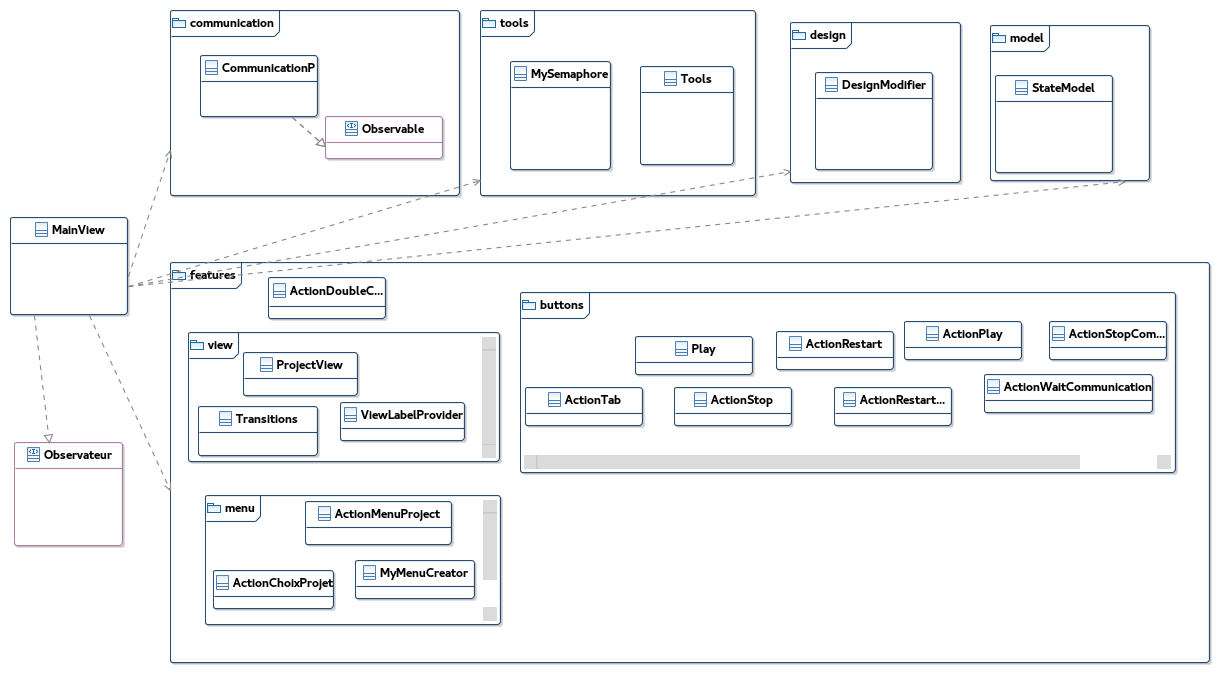
\includegraphics[width=\linewidth]{umlClassDiagram}
  \caption{plugin class diagram}
  \label{fig:classDiagram}
\end{figure}



\section{Functionality implemented}

During this project I had time to implements a lot of functionality for the simulation.


On the figure \ref{fig:result}, you can see the result of my project. It is an Eclipse view, on the top there is a list of all transition possible, and on the bottom it is a tree of the project view. The tree has at the top the name of the project simulated, then the name of all class, end to finish the name of all instances.

\begin{figure}[h]
  \centering
  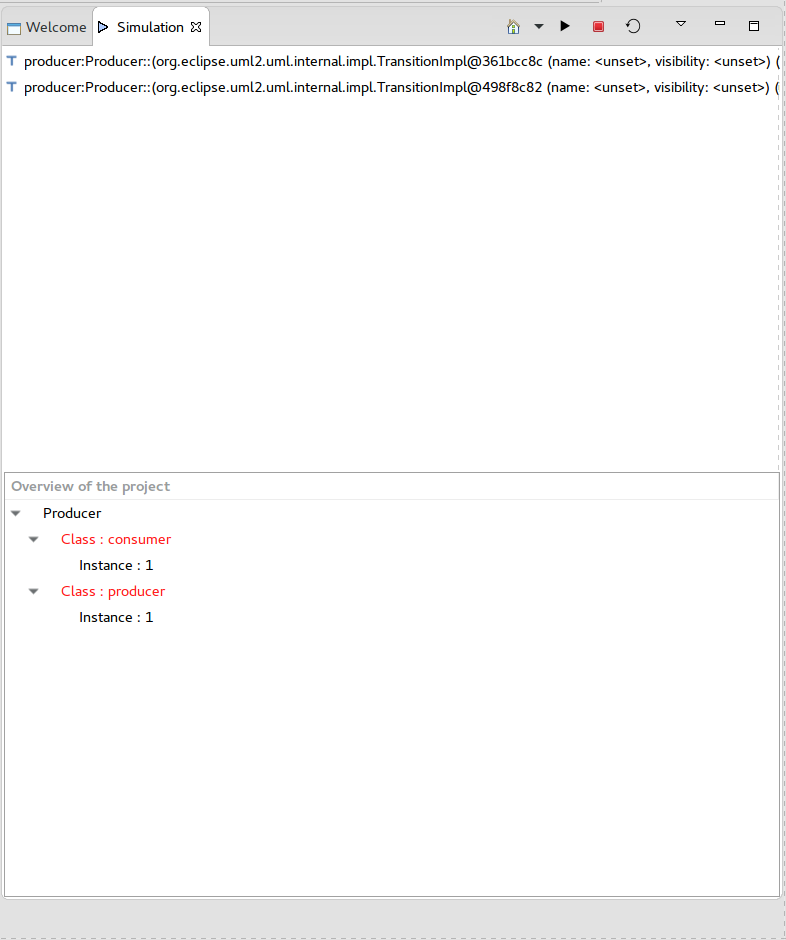
\includegraphics[width=0.4\linewidth]{result}
  \caption{result in \umld}
  \label{fig:result}
\end{figure}

On the top, if the user click on a transition this transition is selected as the next transition, On the bottom, if he click on an instance of a class it is chosen as the visible instance of the model, and if he click on the class name all instances of this class are visible (useful only if there is multiple instance for a same class). Current instances visible are in red.
~\\

On the top, it is possible to see that there is many button. These buttons create some action:

\noitemsep
\begin{description}
\item[home] permit to change the project that we want to simulated
\item[play] launch a simulation where a random step is chosen every 1s.
\item[stop] stop the simulation launch with play
\item[replay] restart the simulation of the project
\item[menu] contain all previous buttons but also:
  \begin{description}
  \item[stop simulator] stop the communication with current simulator
  \item[wait a simulator] start a new server and wait a communication of a new simulator
  \item[restart simulator] restart a communication with the default simulator
  \end{description}
\end{description}
\doitemsep


To finish, I implemented the possibility to see the current state of all state machine diagram in the UML model. You can see on the figure \ref{fig:result2} a test that I did on one model given by Ciprian Teodorov. The red state is the current state.

\begin{figure}[h]
  \centering
  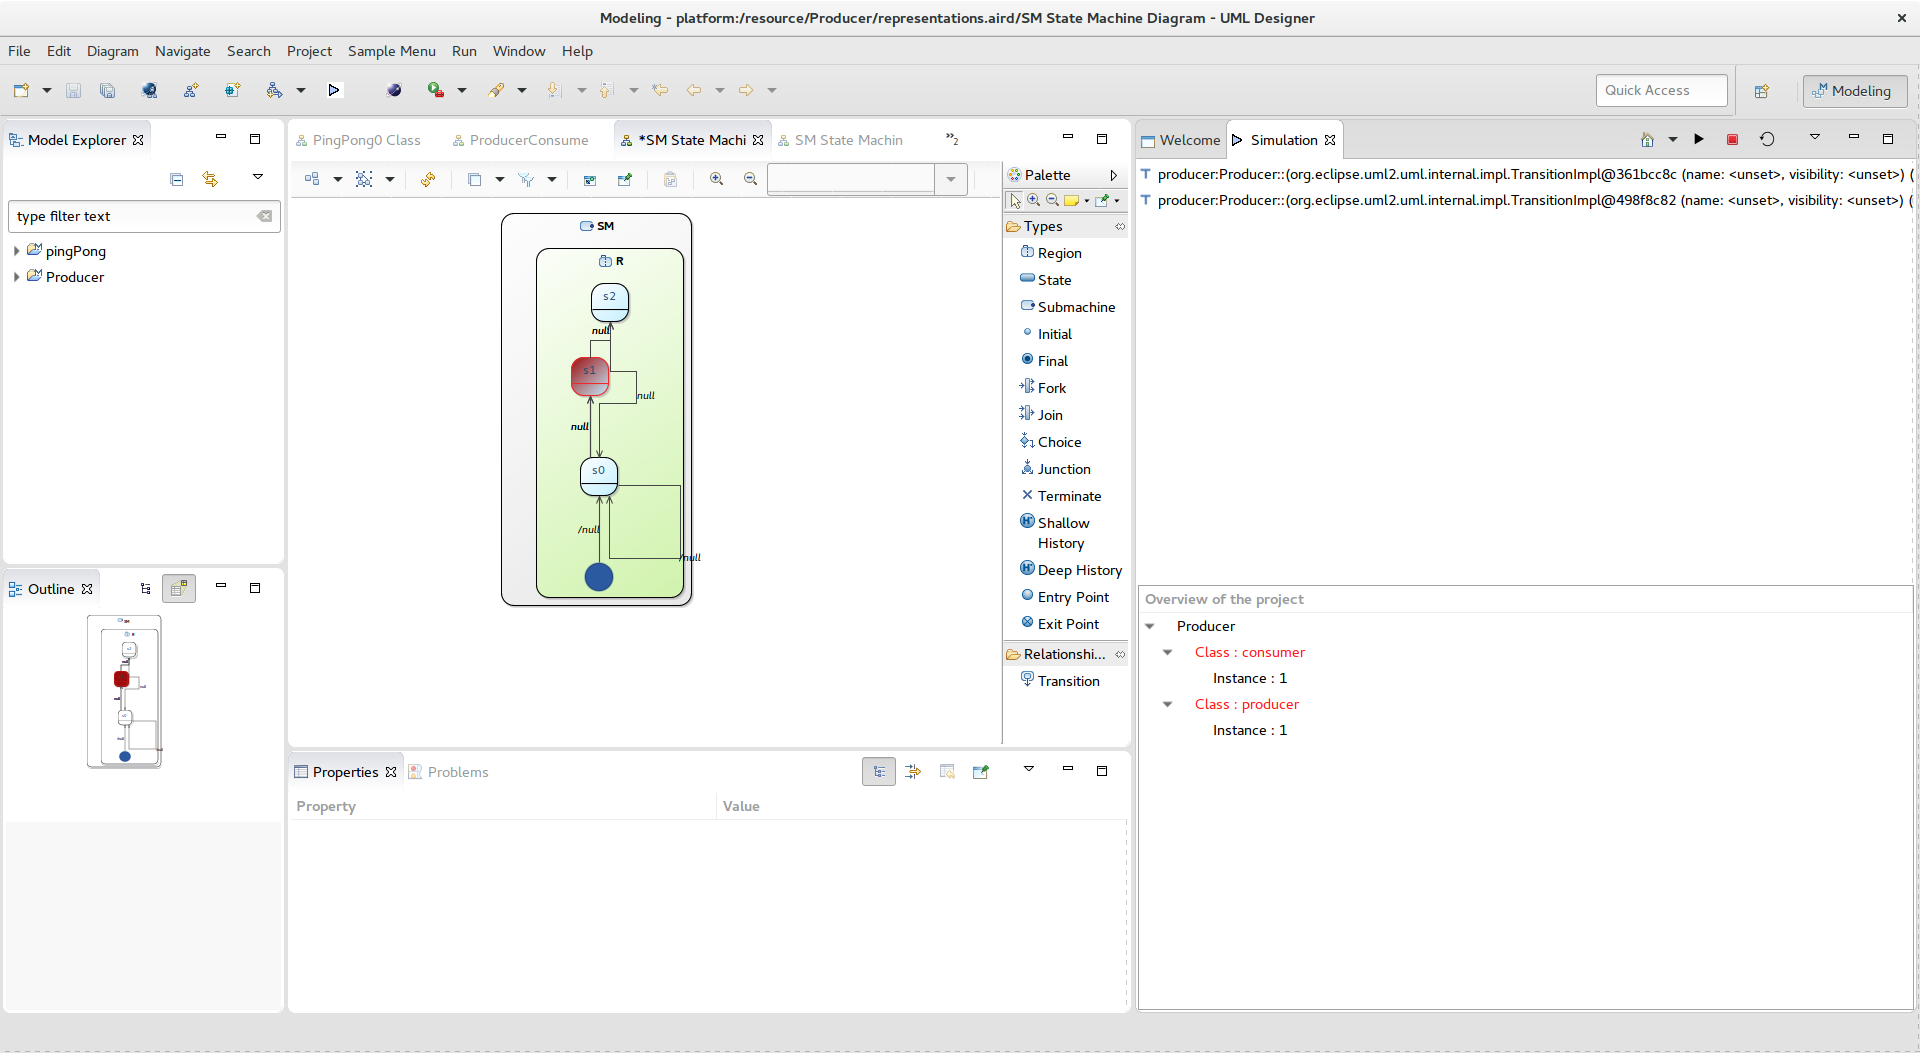
\includegraphics[width=\linewidth]{umldsimulator2}
  \caption{result of a simulation}
  \label{fig:result2}
\end{figure}


% I am going to present the result of my work. If you want a better description of the problems and the choice taken you can read the appendix ???.


% \section{Plugin}

% First I will talk about the plugin. The plugin is the part which realize the display in \umld and the communication to the layer of the simulator. \umld is based on Eclipse so to realize the plugin I realize a Eclipse plugin.
% ~\\



%%% Local Variables:
%%% mode: latex
%%% TeX-master: "../rapport_de_base"
%%% End:
